\newpage

\section{Ableitungen}

\subsection{Geometrische Interpretation}
Der Differenzquotient entspricht der Steigung einer Sekanten des Graphen der
Funktion $f$, die Ableitung entspricht der Steigung der Tangente 
(bei($x_0, f(x_0))$).

\begin{center}
    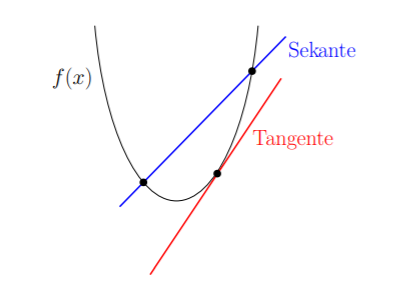
\includegraphics[width=0.5\linewidth]{images/ableitungen.png}
\end{center}

\subsection{Die Ableitungsfunktion}
\[
    f'(x), \frac{df}{dx}, \frac{dy}{dx}
\]
Bei gegebener Funktion $f(x) = c$ gilt $f'(x)=0$ für jedes $x \in \mathbb{R}$. \\
Bei gegebener Funktion $f(x)=x^k$ mit $k\neq 0$ gilt $f'(x)=k \cdot x^{k-1}$. \\
\\
Die \textit{zweite Ableitung} erhält man, indem man die Ableitungsfunktion noch einmal ableitet. Die dritte in dem man die zweite noch einmal ableitet und so weiter.

\subsection{Ableitungsregeln}
\subsubsection{Faktorregel}
\[
    (c \cdot f)'(x) = c \cdot f'(x)
\]
\textbf{Beispiel: } $(4x^3)'=4 \cdot (x^3)' = 4 \cdot 3x^2 = 12x^2$

\subsubsection{Summenregel}
\[
    (f+g)'(x) = f'(x) + g'(x)
\]
\textbf{Beispiel: } $(7x^5-3x^3+5x^2-14x+6)' = (7x^5)' - (3x^3)' + (5x^2)' - (14x)' + (6)' = 35x^4-9x^2+10x-14$

\subsubsection{Produkteregel}
\[
    (u \cdot v)'(x) = u'(x) \cdot v(x) + u(x) \cdot v'(x)
\]
\textbf{Beispiel: }  $f(x) = ((3x^3 + x^2)(4x^2+1))$. Gesucht: $f'(x)$.
\begin{align*}
    &u = 3x^3 + x^2, u'=9x^2 + 2x \\
    &v=4x^2+1, v'=8x \\
    &\Rightarrow f'(x) = u'v + uv' = (9x^2+2x)(4x^2+1)+(3x^3+x^2) \cdot 8x \\
    &= 36x^4 + 9x^2 + 8x^3 + 2x + 24x^4 + 8x^3 = 60x^4 + 16x^3 + 9x^2 + 2x
\end{align*}

\subsubsection{Quotientenregel}
\[
    (\frac{u}{v}')(x)=\frac{u'(x) \cdot v(x) - u(x) \cdot v'(x)}{(v(x))^2}
\]
\textbf{Beispiel: } $f(x) = (\frac{3x^2-x}{2x^3+1})$. Gesucht: $f'(x)$.
\begin{align*}
    &u = 3x^2-x, u' = 6x-1 \\
    &v = 2x^3+1, v' = 6x^2 \\
    &\Rightarrow f'(x) = \frac{u'v = uv'}{v^2} = \frac{(6x-1)\cdot (2x^3 + 1)- (3x^2-x) \cdot 6x^2}{(2x^3+1)^2}
\end{align*}

\subsubsection{Kettenregel}
\[
    (F \circ u)'(x) = F'(u) \cdot u'(x) \\
\]
\textbf{Beispiel: }
\begin{align*}
    &f(x)=(x^3+4)^{-2} \\
    &F(u) = u^{-2}, F'(u)=-2u^{-3} \\
    &u(x) = (x^3+4), u'(x)=3x^2 \\
    &\Rightarrow f'(x)=-2u^{-3} \cdot 3x^2 = -2(x^3 + 4)^{-3} \cdot 3x^2
\end{align*}

\subsubsection{Ableitungen bestimmter Funktionen}
\begin{itemize}
    \item $(\sin(x))'= \cos(x)$
    \item $(\cos(x))'= -\sin(x)$
    \item $(e^x)'= e^x$
    \item $(a^x)'= a^x \cdot \ln(a)$
    \item $(\ln(x))'= \frac{1}{x}$
    \item $(\log_a(x))'= \frac{1}{x \cdot \ln(a)}$
\end{itemize}

\subsection{Differenzierbarkeit}
Eine Funktion $f(x)$ ist an der Stelle $x_0$ differenzierbar, wenn die linksseitige mit der rechtsseitigen Ableitung übereinstimmt.
Eine Funktion $f(x)$ heisst ableitbar, wenn die Ableitung an jeder Stelle ihres Definitionsbereichs definiert ist.

\begin{center}
    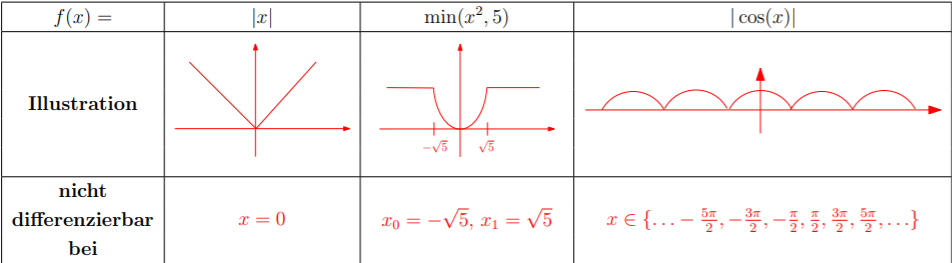
\includegraphics[width=1\linewidth]{images/differenzierbarkeit_beispiele.png}
\end{center}

\vfill

\subsection{Linearisierung einer Funktion}
Die Funktionsgleichung für die Tangente von $f(x)$ an der Stelle $x_0$ lautet:
\[
    y = f'(x_0) \cdot (x - x_0) + f(x_0)
\]

\subsubsection{Newton Verfahren}
\[
    x_{n+1} = x_n - \frac{f(x_n)}{f'(x_n)}
\]
\textbf{Beispiel: } $f(x) = x^3 + 5x -4$
\begin{center}
    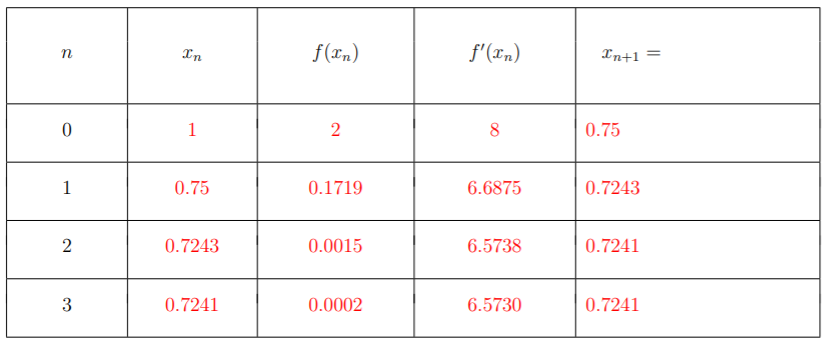
\includegraphics[width=1\linewidth]{images/newton.png}
\end{center}

\subsubsection{Fixpunkte des Newton-Verfahrens}
Unter einem Fixpunkt $\phi (x)$ versteht man ein $x$ mit $\phi (x) = x$. \\
Unter einem Fixpunkt des Newton-Verfahrens versteht man einen Wert $x$ mit folgender Eigenschaft: Ist $x_n = x$, so ist $x_{n+1} = x_n = x$. \\
Fixpunkte sind also alle Werte $x$ mit der Eigenschaft $x=x-\frac{f(x)}{f'(x)}$. \\
Startet man das Newton-Verfahren mit einem Wert $x_0$ in der Nähe eines Fixpunktes, so strebt das Verfahren gegen diesen Fixpunkt.